\documentclass[8pt]{beamer}
% \usepackage[utf8]{inputenc} is no longer required (since 2018)

%Set the font (output) encoding
%--------------------------------------
\usepackage[T1]{fontenc} %Not needed by LuaLaTeX or XeLaTeX

%French-specific commands
%--------------------------------------
\usepackage[french]{babel}
\usepackage[autolanguage]{numprint} % for the \nombre command

%Hyphenation rules
%--------------------------------------
\usepackage{hyphenat}
\hyphenation{mate-mática recu-perar}
%--------------------------------------
\usepackage{amsmath}
\usepackage{bm}
\usepackage{subcaption}
\usepackage{tikz}
\usepackage{wasysym}
\usepackage{fontawesome5}
\usepackage{svg}

% Theme choice
\usetheme[block=fill, sectionpage=none, progressbar=frametitle,
    numbering=none]{metropolis}

\usecolortheme{orchid}

% Title, author, and date information
\title{Gestion de la Mémoire dans les Systèmes Informatiques}
\subtitle{Hiérarchie de la Mémoire et Pagination}
\author{Yohan Chatelain}
\institute{Polytechnique Montr\'eal}
\date{3 juin 2024}

\begin{document}

% Title slide
\begin{frame}
    \titlepage
\end{frame}

\begin{frame}{Plan du cours}
    \begin{figure}
        \centering
        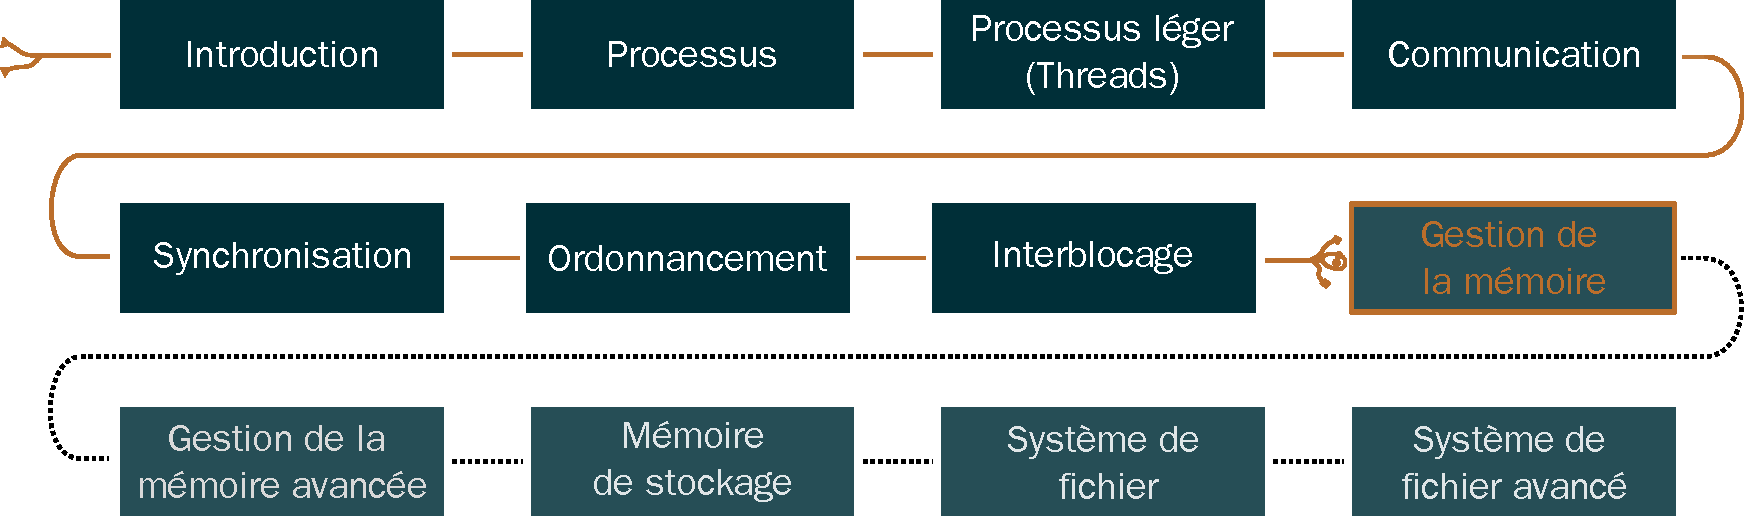
\includegraphics[width=\textwidth]{figures/plan_cours.pdf}
    \end{figure}
    \vfill
    \begin{block}{Objectifs : }

        \begin{itemize}
            \item Les différents types de mémoires
            \item La hiérarchie de la mémoire
            \item La gestion de la mémoire par pagination
        \end{itemize}
    \end{block}
\end{frame}

\addtocounter{framenumber}{-2}
\setbeamertemplate{frame numbering}[fraction]

\section*{Introduction}
\begin{frame}
    \frametitle{Introduction}
    \begin{itemize}
        \item La mémoire est le deuxième composant majeur de tout ordinateur
    \end{itemize}
    \begin{figure}
        \centering

        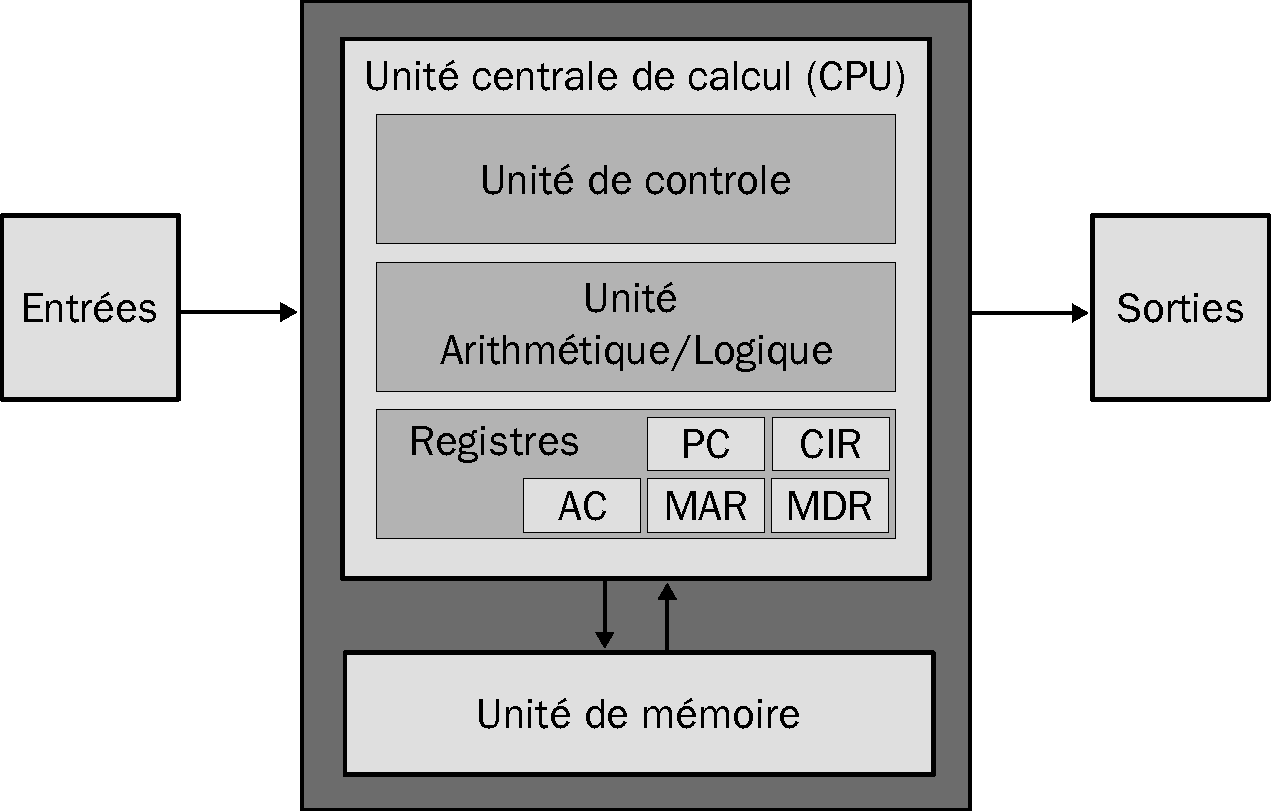
\includegraphics[width=.45\textwidth]{figures/Von-Neumann-Architecture-Diagram.pdf}
        \subcaption{Architecture de Von Neumann~\cite{tanenbaum2009modern}}
        \label{fig:sub1}
    \end{figure}
    \begin{block}{La mémoire idéale devrait être :}
        \begin{itemize}
            \item Extrêmement rapide
            \item De très grande capacité
            \item Peu coûteuse
        \end{itemize}
    \end{block}

\end{frame}

\begin{frame}{Spoiler alert!}
    \begin{figure}
        \centering
        
\includegraphics[width=0.5\textwidth]{figures/meme.png}
        \label{fig:memory_speed}
    \end{figure}

    \begin{alertblock}{Problème}
        \begin{itemize}
            \item La technologie actuelle ne satisfait pas tous ces objectifs
        \end{itemize}
    \end{alertblock}
\end{frame}

\begin{frame}
    \frametitle{Les différents types de mémoires}
    \begin{alertblock}{Questions :}
        \begin{itemize}
            \item Quels types de m\'emoires connaissez-vous ?
            \item Quel est le r\^ole de chacune de ces m\'emoires ?
            \item Comment ces m\'emoires sont-elles organis\'ees ?
        \end{itemize}
    \end{alertblock}
\end{frame}

\begin{frame}
    \frametitle{Les différents types de mémoires}
    \begin{block}{Principe général}
        \begin{itemize}
            \item M\'emoire rapide $\implies$ plus  ch\`ere \`a
                  fabriquer $\implies$ capacité  limit\'ee
            \item Chaque m\'emoire r\'epond \`a un objectif en
                  terme de rapidit\'e/capacité/co\^ut
        \end{itemize}
    \end{block}
    \begin{enumerate}
        \item \textbf{Registre} : Mémoire très rapide, très coûteuse et
              volatile. \\
              Contient les données de travail des unités de calculs.
        \item \textbf{Cache} : Mémoire rapide, coûteuse et volatile. \\
              Contient les données et instructions les plus utilisées par les
              unités de calculs.
        \item \textbf{Centrale} : Mémoire de vitesse moyenne, coût moyen et
              volatile. \\
              Contient les données et instructions des programmes en cours
              d'exécution
        \item \textbf{Stockage} : Mémoire lente, peu coûteuse et non volatile
              \\
              Contient les données et instructions des programmes non utilisés
              \\
    \end{enumerate}

\end{frame}

\begin{frame}{Hiérarchie de la mémoire}

    \begin{figure}
        \centering
        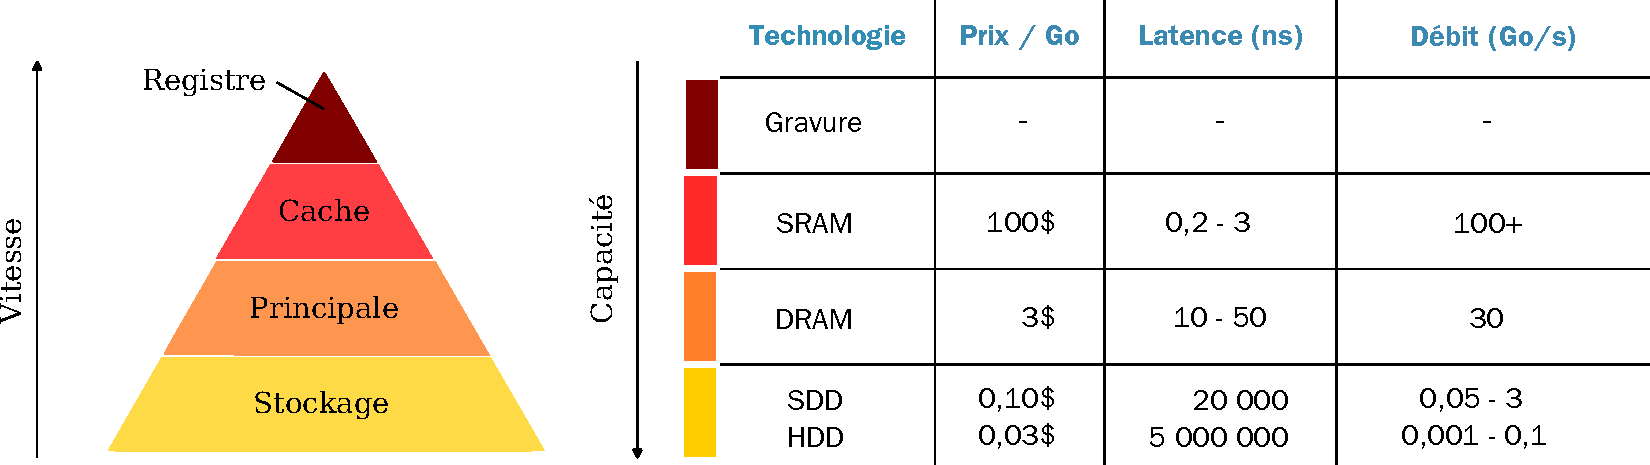
\includegraphics[width=\linewidth]{figures/hierarchy_memory.pdf}
        \caption{Hiérarchie de la mémoire (adapté de~\cite{harris2021digital})}
    \end{figure}

    \textbf{Principe de localité}
    \begin{itemize}
        \item Les programmes ont tendance à accéder aux \textbf{données} et
              \textbf{instructions} selon deux principes :
              \begin{enumerate}
                  \item \textbf{Localité temporelle} : Acc\`es consécutifs
                        (sans interruptions) aux
                        mêmes données ou instructions
                  \item \textbf{Localité spatiale} : Acc\`es à des données
                        contiguës (proches les unes des autres) en mémoire
              \end{enumerate}
        \item Il convient donc de garder les données fréquemment utilisées
              rapidement accessible par le processeur (proche du processeur)
    \end{itemize}
\end{frame}

\begin{frame}{Hiérarchie de la mémoire - Représentation au niveau du SE}
    \begin{onlyenv}<1>
        \begin{figure}
            \centering

            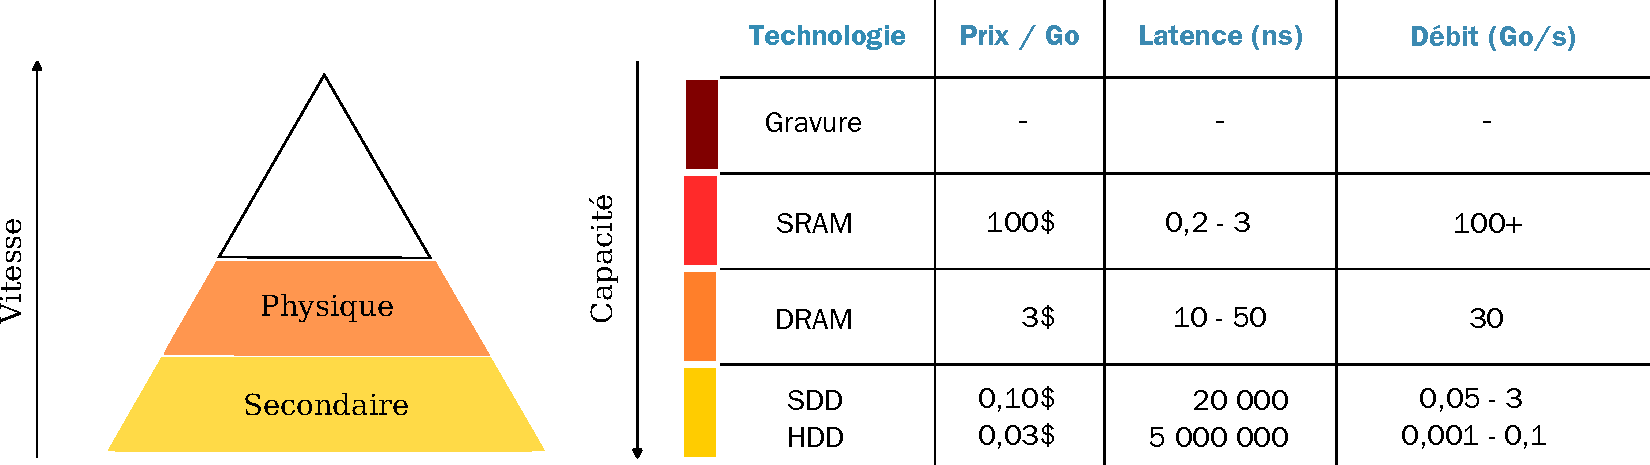
\includegraphics[width=\linewidth]{figures/hierarchy_memory_virtual.pdf}
            \caption{Hiérarchie de la mémoire (adapté
                de~\cite{harris2021digital})}
        \end{figure}
    \end{onlyenv}
    \begin{onlyenv}<2>
        \begin{figure}
            \centering

            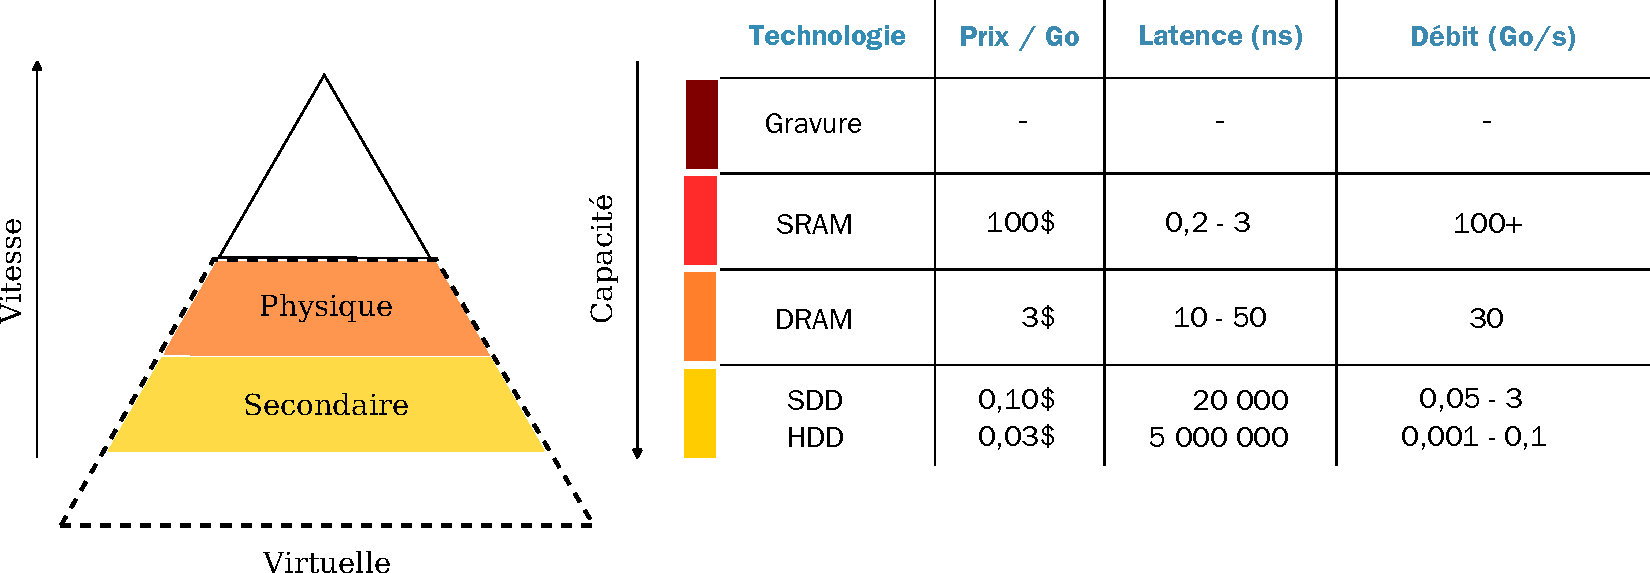
\includegraphics[width=\linewidth]{figures/hierarchy_memory_virtual_physic.pdf}
            \caption{Hiérarchie de la mémoire (adapté
                de~\cite{harris2021digital})}
        \end{figure}
    \end{onlyenv}

    \textbf{La représentation de la mémoire :}
    \begin{enumerate}
        \item \textbf{Mémoire Physique} : Mémoire centrale qui contient
              les
              données et instructions des programmes en cours d'exécution
        \item \textbf{Mémoire Secondaire} : Mémoire d'appoint qui
              contient
              les données et instructions des programmes non utilisés
        \item<2> \textbf{Mémoire Virtuelle} : Vision unifiée de la
            mémoire

    \end{enumerate}
\end{frame}

\begin{frame}[c]
    \frametitle{Mémoire Virtuelle - Illustration}
    \begin{onlyenv}<1>
        \vspace*{1.25cm}
        \begin{figure}
            \centering

            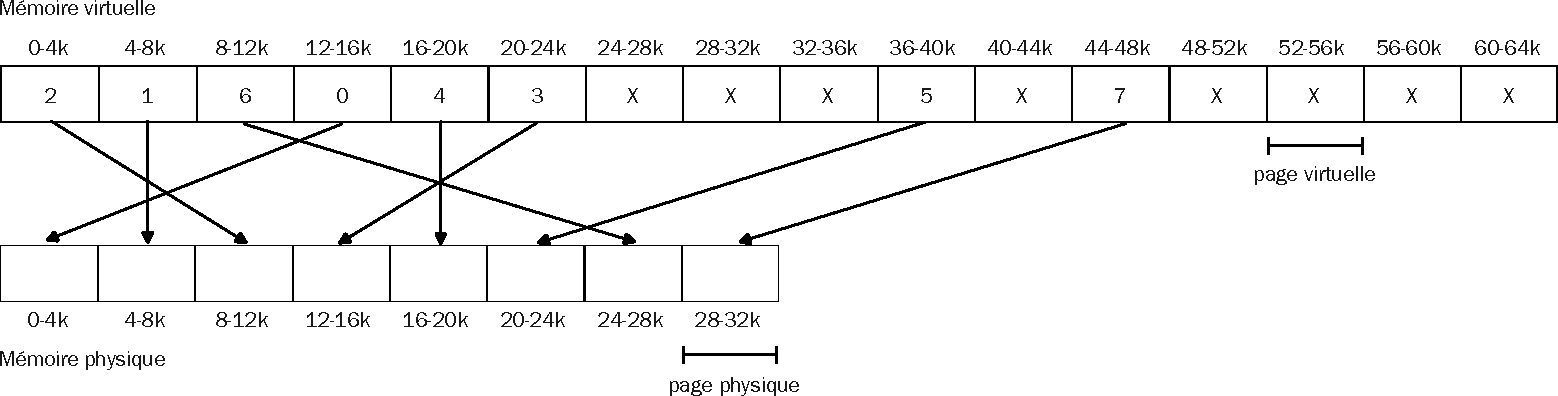
\includegraphics[height=.25\textwidth]{figures/memoire_virtuelle_physique.pdf}
            \subcaption{Diagramme de la mémoire
                virtuelle et la mémoire physique (adapté
                de~\cite{tanenbaum2009modern})}
        \end{figure}
    \end{onlyenv}
    \begin{exampleblock}{Architecture 16bits}
        \begin{itemize}
            \item  $2^{16}$ adresses possibles, soit 64ko
                  (1Ko=$2^{10}$o) adressable virtuellement
            \item Une configuration de 32ko de RAM + 64ko de disque
            \item M\'emoire physique : 32ko, M\'emoire virtuelle : 64ko
            \item Espace d'adressage 32ko = $32 \times 2^{10} = 2^5
                      \times2^{10} = 2^{15}$o $\to$ 15 bits n\'ecessaires
        \end{itemize}
    \end{exampleblock}
\end{frame}

\begin{frame}
    \frametitle{Mémoire Virtuelle}
    \begin{block}{Principes}
        \begin{itemize}
            \item \textbf{Abstraction} de la mémoire physique et secondaire par
                  le système d'exploitation
            \item Permet de \og{virtuellement}\fg{} augmenter la capacité de la
                  \textbf{mémoire physique}
            \item Illusion d’un \textbf{espace mémoire
                      contigu} de grande capacité au programmeur
            \item Chaque processus \`a son \textbf{propre espace
                      d'adresses}
            \item La mémoire virtuelle est divisée en \textbf{pages}
        \end{itemize}
    \end{block}
\end{frame}

\begin{frame}[c]
    \frametitle{Mémoire Virtuelle - Illustration}
    \begin{figure}
        \centering

        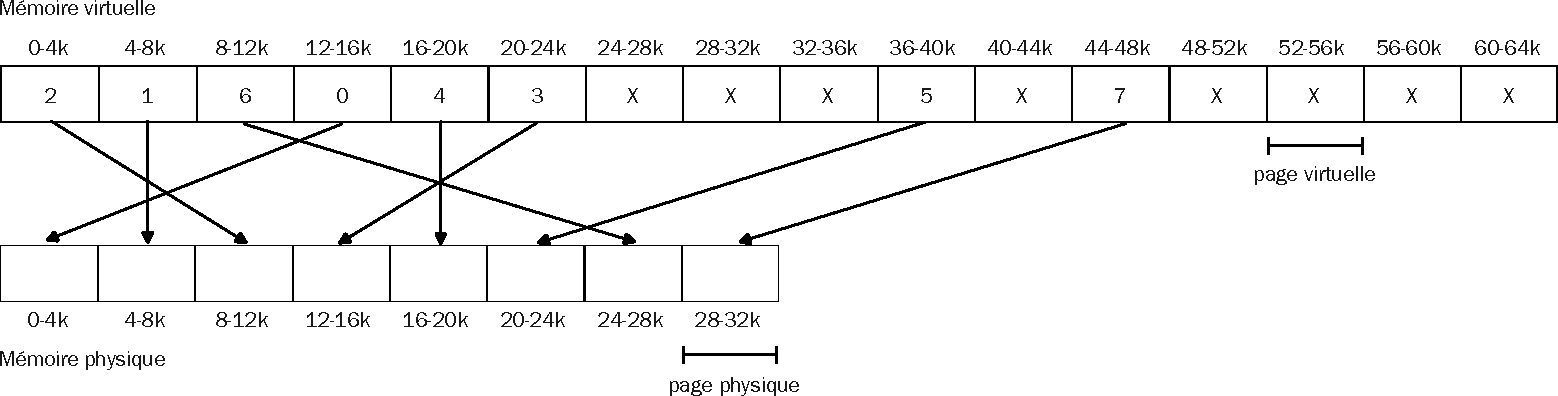
\includegraphics[width=\textwidth]{figures/memoire_virtuelle_physique.pdf}
        \subcaption{Diagramme de la mémoire
            virtuelle et la mémoire physique (adapté
            de~\cite{tanenbaum2009modern})}
    \end{figure}
    \begin{alertblock}{Question : }
        \begin{itemize}
            \item
                  Quelle est l'avantage du d\'ecoupage en pages ?
        \end{itemize}
    \end{alertblock}
    \pause
    \begin{exampleblock}{Solution :}
        \begin{itemize}
            \item Un processus \textbf{n'utilise pas toute la mémoire} qui
                  lui est
                  allouée en même
                  temps
            \item Charger en mémoire \textbf{uniquement les pages nécessaires}
                  à
                  l'exécution
            \item Principe de \textbf{localité}
        \end{itemize}
    \end{exampleblock}

\end{frame}

\begin{frame}{La Pagination}
    \begin{block}{D\'efinition}
        \begin{itemize}
            \item \textbf{Pagination} : Division de la mémoire V/P	en
                  blocs de taille fixe appelés \textbf{pages}
            \item \textbf{Page} : Bloc de mémoire V/P de \textbf{taille fixe}
                  (4-64ko)
            \item \textbf{Table de Pages} : Associe les \textbf{pages
                      virtuelles} aux \textbf{pages physiques}
        \end{itemize}
        V/P : Mémoire Virtuelle / Mémoire Physique
    \end{block}
\end{frame}

\begin{frame}
    \frametitle{Table des pages et Traduction}
    \begin{figure}
        \begin{minipage}[b]{0.45\linewidth}
            \centering

            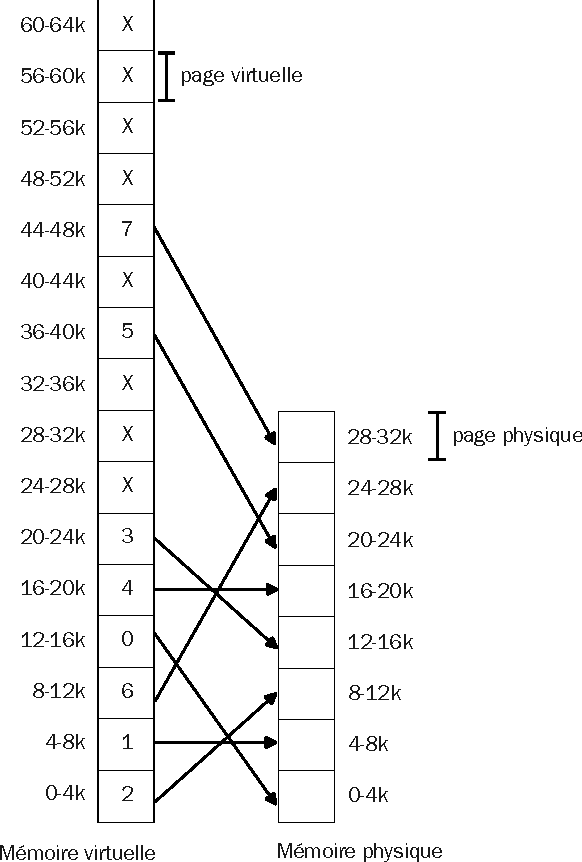
\includegraphics[width=.75\linewidth]{figures/memoire_virtuelle_physique_T.pdf}
            \subcaption{}
            \label{fig:page_table}
        \end{minipage}
        \begin{minipage}[b]{0.5\linewidth}
            \centering
            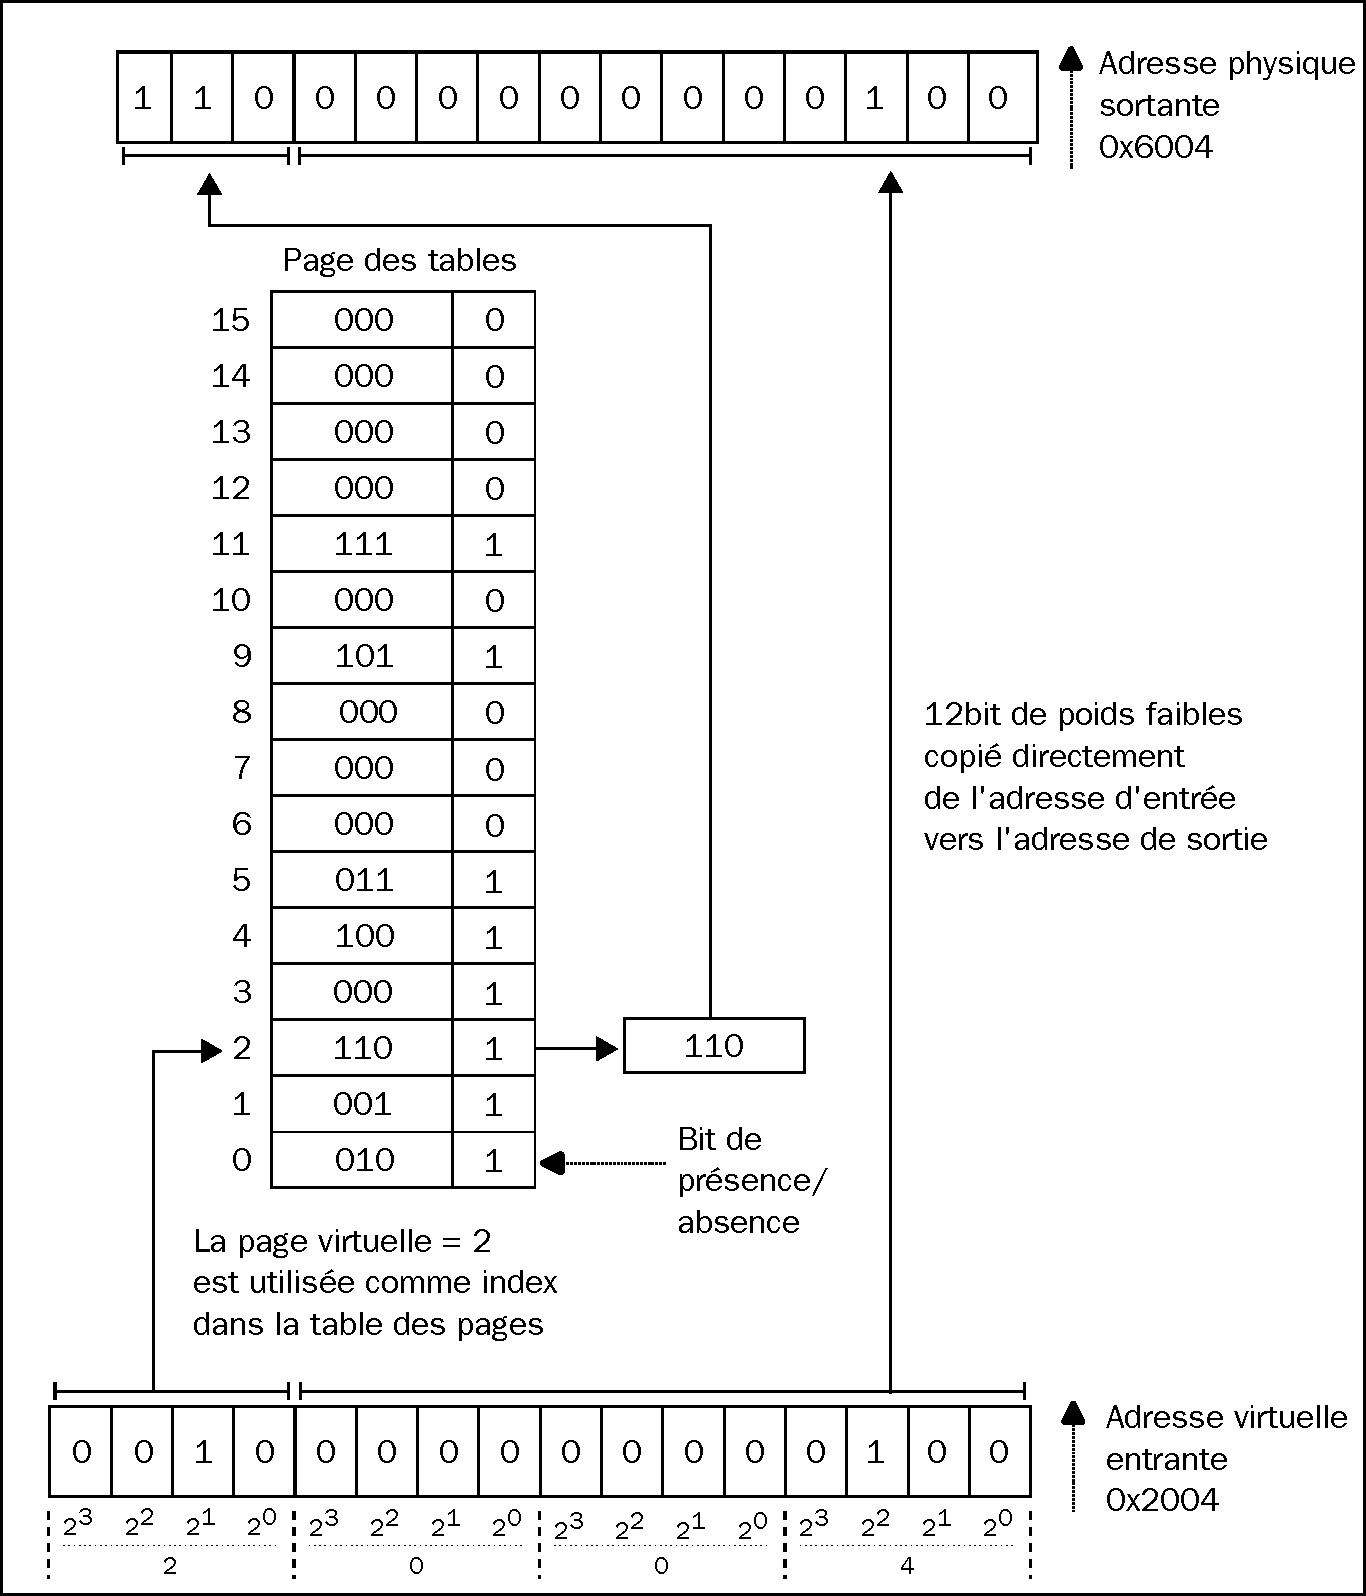
\includegraphics[width=.95\linewidth]{figures/page_mapping.pdf}
            \subcaption{}
            \label{fig:page_mapping}
        \end{minipage}
        \caption{Table des pages simplifiée pour une architecture 16 bits avec
            un bit de
            pr\'esence. \\ (a) Table des pages et (b) Traduction mémoire
            virtuelle vers physique~(adaptée de \cite{tanenbaum2009modern}).
            Architecture 16 bits,
            Mémoire Virtuelle : 64ko, Mémoire Physique : 32ko,
            Taille de page : 4ko. \\
        }
    \end{figure}
    % $\to$ Le\c{c}on X pour des tables des pages plus complexe.

    % \includegraphics[width=\linewidth]{memory_mapping_example}
\end{frame}

\begin{frame}{Conclusion}
    \begin{block}{Mémoire dans les systèmes informatiques}
        \begin{itemize}
            \item Les différents \textbf{types de mémoires} sont
                  \begin{itemize}
                      \item registres, caches, mémoire centrale et mémoire de
                            masse
                  \end{itemize}
            \item La \textbf{hiérarchie de la mémoire} :
                  \begin{itemize}
                      \item divise la mémoire en niveaux de rapidité et de
                            capacité
                            %   \item est une solution aux contraintes de
                            %         \textbf{rapidité},
                            %         \textbf{capacité} et \textbf{coût}
                      \item r\'epond au principe de \textbf{localité}
                  \end{itemize}
            \item La gestion de la mémoire par \textbf{pagination} :
                  \begin{itemize}
                      \item utilise la \textbf{mémoire virtuelle} pour allouer
                            plus de
                            mémoire que la mémoire physique
                      \item divise la mémoire virtuelle en \textbf{pages}
                      \item utilise une \textbf{table des pages} pour
                            \textbf{traduire} les
                            adresses
                            virtuelles en adresses physiques
                  \end{itemize}
        \end{itemize}
    \end{block}
    % \begin{exampleblock}{Prochaines leçons}
    %     \begin{itemize}
    %         \item Politiques de placement dans les caches
    %         \item Politiques de remplacement et d'\'ecriture dans les caches
    %         \item Tables de pages avancées (multi-niveaux, inversion de pages)
    %         \item Algorithmes de remplacement de pages
    %         \item * Les différents types de mémoires
    %         \item * La hiérarchie de la mémoire
    %         \item * La gestion de la mémoire par pagination

    %     \end{itemize}
    % \end{exampleblock}
\end{frame}

\setbeamertemplate{frame numbering}[none]

\bibliographystyle{apalike}
\begin{frame}{Bibliographie}
    \nocite{*}
    \bibliography{main}
\end{frame}
\addtocounter{framenumber}{-1}

\end{document}
